%===============================================================================
%===============================================================================
%
\clearpage
%
\subsection{Example-0404-c \texttt{[PLAUSIBLE]}}
%
%===============================================================================
%
\subsubsection{Mathematical model}
%
We solve the Monodomain Equation
%
\begin{align}
    \sigma \Delta V_m(t) = A_m\Big(C_m \dfrac{\partial V_m}{\partial t} + I_{ionic}(V_m)\Big) & &&\Omega = [0, 1], \quad t \in [0, 10.0]
\end{align}
%
where $V_m(t)$ is given by the Hodgkin-Huxley system of ODEs \cite{hodgkin1952propagation}

with Neumann boundary conditions
%
\begin{align}
    \dfrac{\partial u}{\partial n} = 0 & &&x = 0,\\
    \dfrac{\partial u}{\partial n} = 0 & &&x = 1.
\end{align}
%
and initial values 
%
\begin{equation*}
  \begin{array}{lll}
    V_m(t=0) = -75
  \end{array}
\end{equation*}
%
Additionally a stimulation current $I_{stim}$ is applied for $t_{stim} = [0, 0.5]$ at the center node of the domain (i.e. at $(x,y) = (\frac12, \frac12,)$).
%

Material parameters:
\begin{equation*}
  \begin{array}{lll}
    \sigma = 3.828\\[4mm]
    A_m = 500\\[4mm]
    C_m = 0.58 \quad \text{for the slow-twitch case,} \quad C_m = 1.0 \quad \text{for the fast-twitch case}\\[4mm]
    I_{Stim} = \begin{cases}
      75/10\cdot(2X) & \text{for } X\geq 10 \text{ reference elements}\\
      75 & \text{for }< \text{ 10 reference elements}\\
    \end{cases}
     \quad \text{for the slow-twitch case,} \\
     \quad I_{Stim} = \begin{cases}
      75/12\cdot(2X) & \text{for } X\geq 12 \text{ reference elements}\\
      75 & \text{for }< \text{ 12 reference elements}\\
    \end{cases}
    \quad \text{for the fast-twitch case}\\[4mm]    
  \end{array}
\end{equation*}
%
%===============================================================================
%
\subsubsection{Computational model}
%
\begin{itemize}
    \item{This example uses generated meshes}
    \item{Commandline arguments are:}
        \subitem{number of elements}
        \subitem{order of interpolation}
        \subitem{solver type (0: direct; 1: iterative)}
        \subitem{time step PDE}
        \subitem{end time}
        \subitem{output file stride}
        \subitem{cellml model file}
        \subitem{if slow-twitch (T: slow-twitch, F: fast-twitch)}
        \subitem{time step ODE}
    \item{Commandline arguments for tests are:}
        \subitem{\verb|64 2 0 0.01 10 5 hodgkin_huxley_1952.cellml F 0.01|}
        \subitem{\verb|64 2 0 0.005 10 10 hodgkin_huxley_1952.cellml F 0.005|}
        \subitem{\verb|64 2 0 0.001 10 50 hodgkin_huxley_1952.cellml F 0.001|}
        \subitem{\verb|64 2 0 0.0005 10 100 hodgkin_huxley_1952.cellml F 0.0005|}
        \subitem{\verb|64 2 0 0.00025 10 200 hodgkin_huxley_1952.cellml F 0.00025|}
    \item{This is a dynamic problem.}
\end{itemize}
%
%===============================================================================
%
\subsubsection{Results}
We run the scenario for different time step widths and examine the experimental order of convergence.
%\begin{figure}[h!]
%    \centering 
%    \includegraphics[width=0.9\columnwidth]{examples/example-0001/doc/figures/analytical_solution.eps} 
%    \caption{Results, analytical solution.}
%    \label{example-0001-analytical-solution-fig}
%\end{figure}
%
%\begin{figure}[h!]
%    \centering 
%    \includegraphics[width=0.9\columnwidth]{examples/example-0001/doc/figures/abaqus_reference.eps} 
%    \caption{Results, Abaqus reference.}
%    \label{example-0001-abaqus-reference-fig}
%\end{figure}
%
%\verbatiminput{examples/example-0001/results/results.summary} % - there are no tests
%\verbatiminput{examples/example-0001/results/failed.tests}
%
\begin{figure}[h!]
    \centering 
    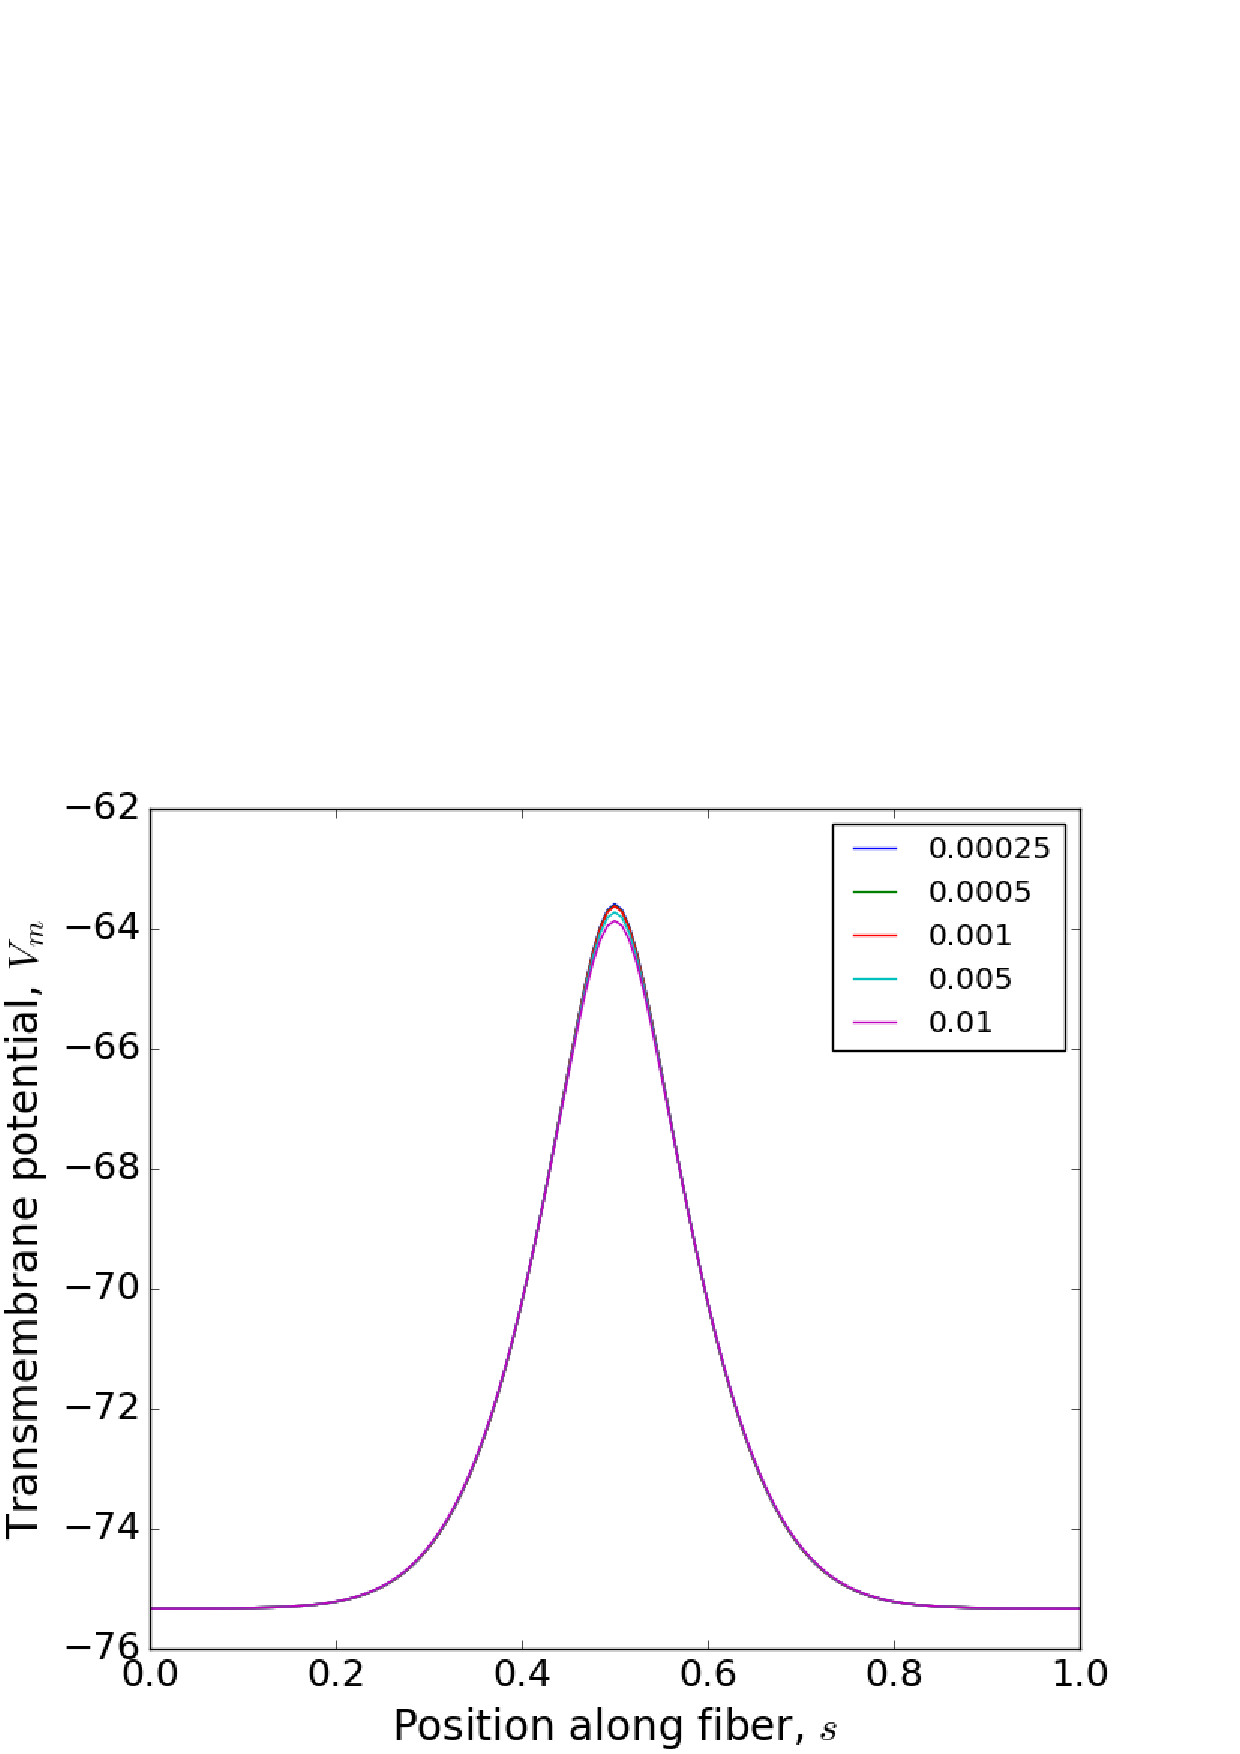
\includegraphics[width=0.9\columnwidth]{examples/example-0404-c/doc/figures/image-Time-Conv-n64-t1.0.png} 
    \caption{$V_m$ for time $t=1.0$, different time step widths ${dt \in \{0.01, 0.005, 0.001, 0.0005, 0.00025\}}$}
    \label{example-0404-c-vm-1.0}
\end{figure}
%
\begin{figure}[h!]
    \centering 
    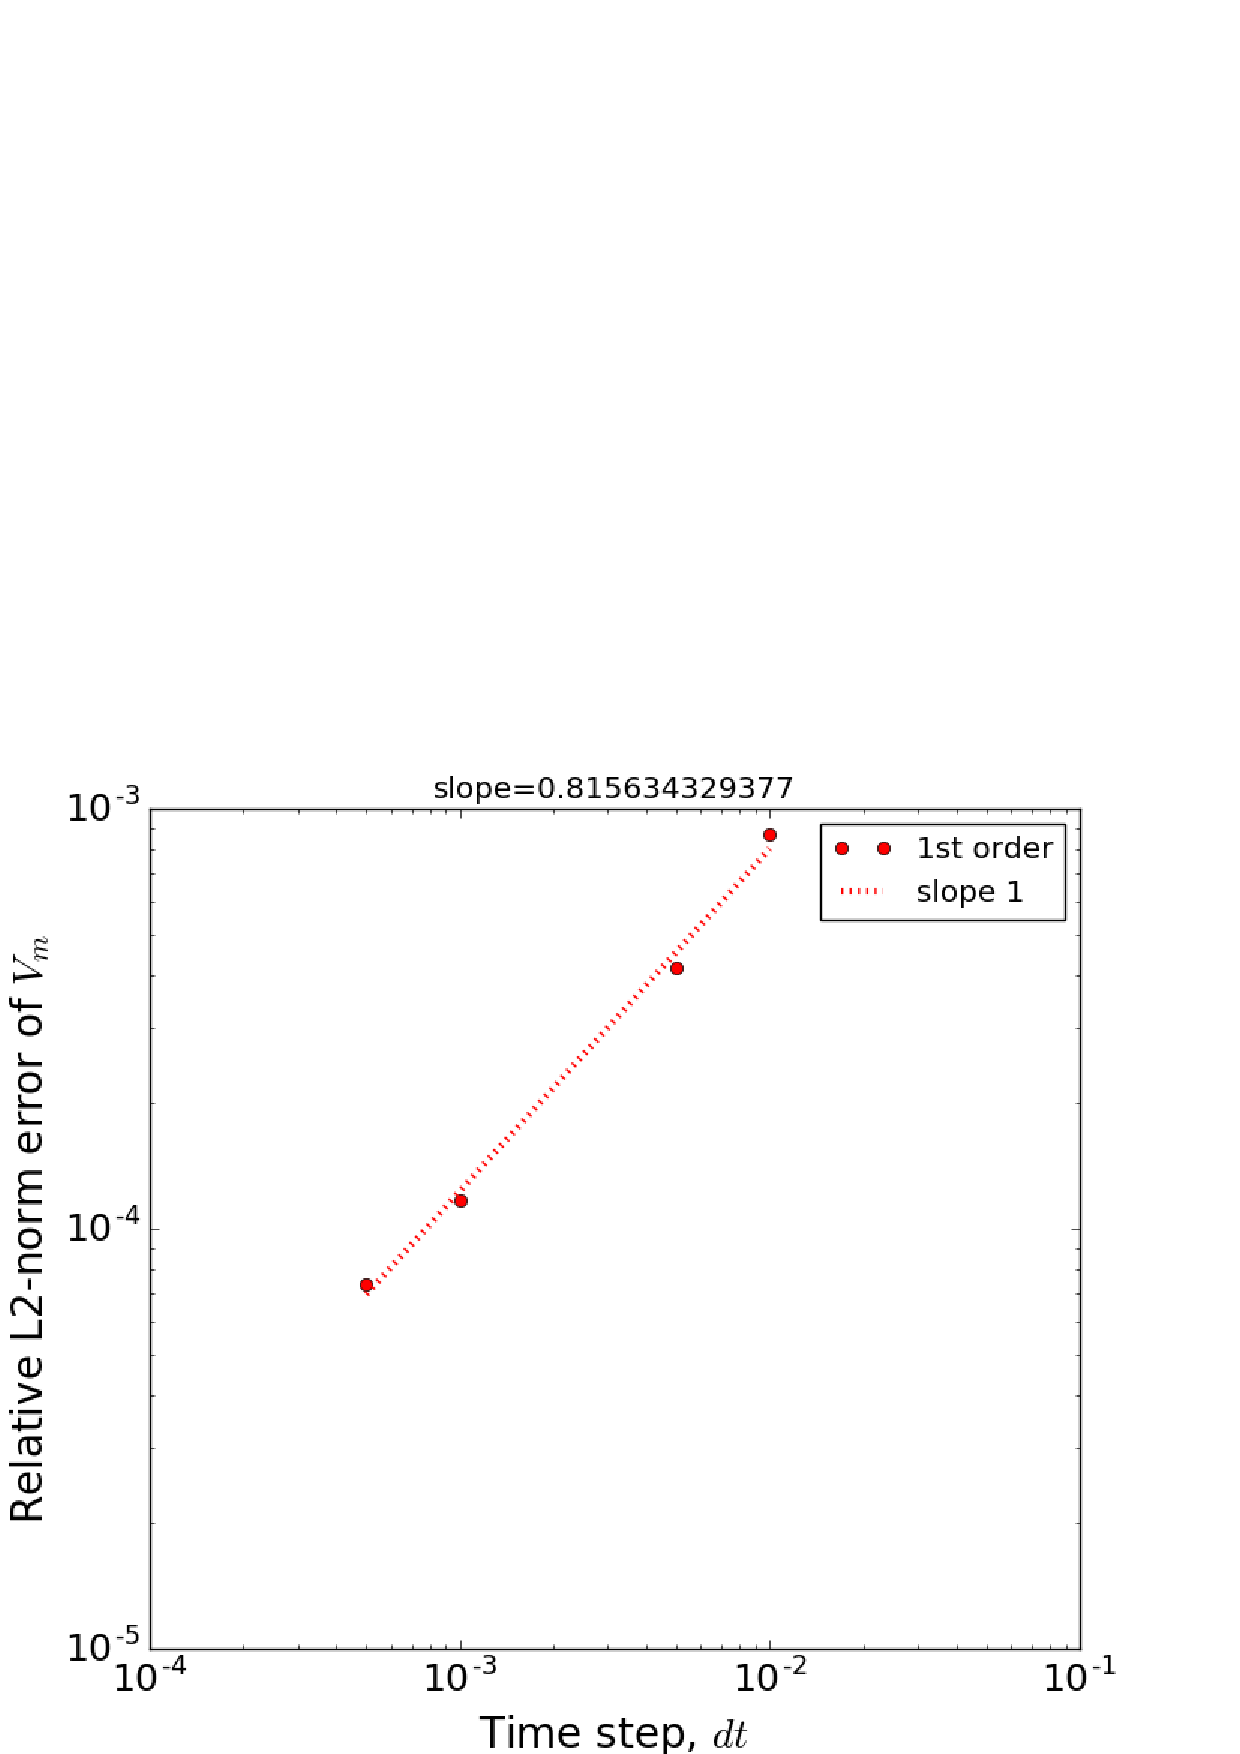
\includegraphics[width=0.9\columnwidth]{examples/example-0404-c/doc/figures/errL2-Time-Conv-n64-t1.0.png} 
    \caption{Error at $t=1.0$ for different time steps widths}
    \label{example-0404-c-error-1.0}
\end{figure}
\begin{figure}[h!]
    \centering 
    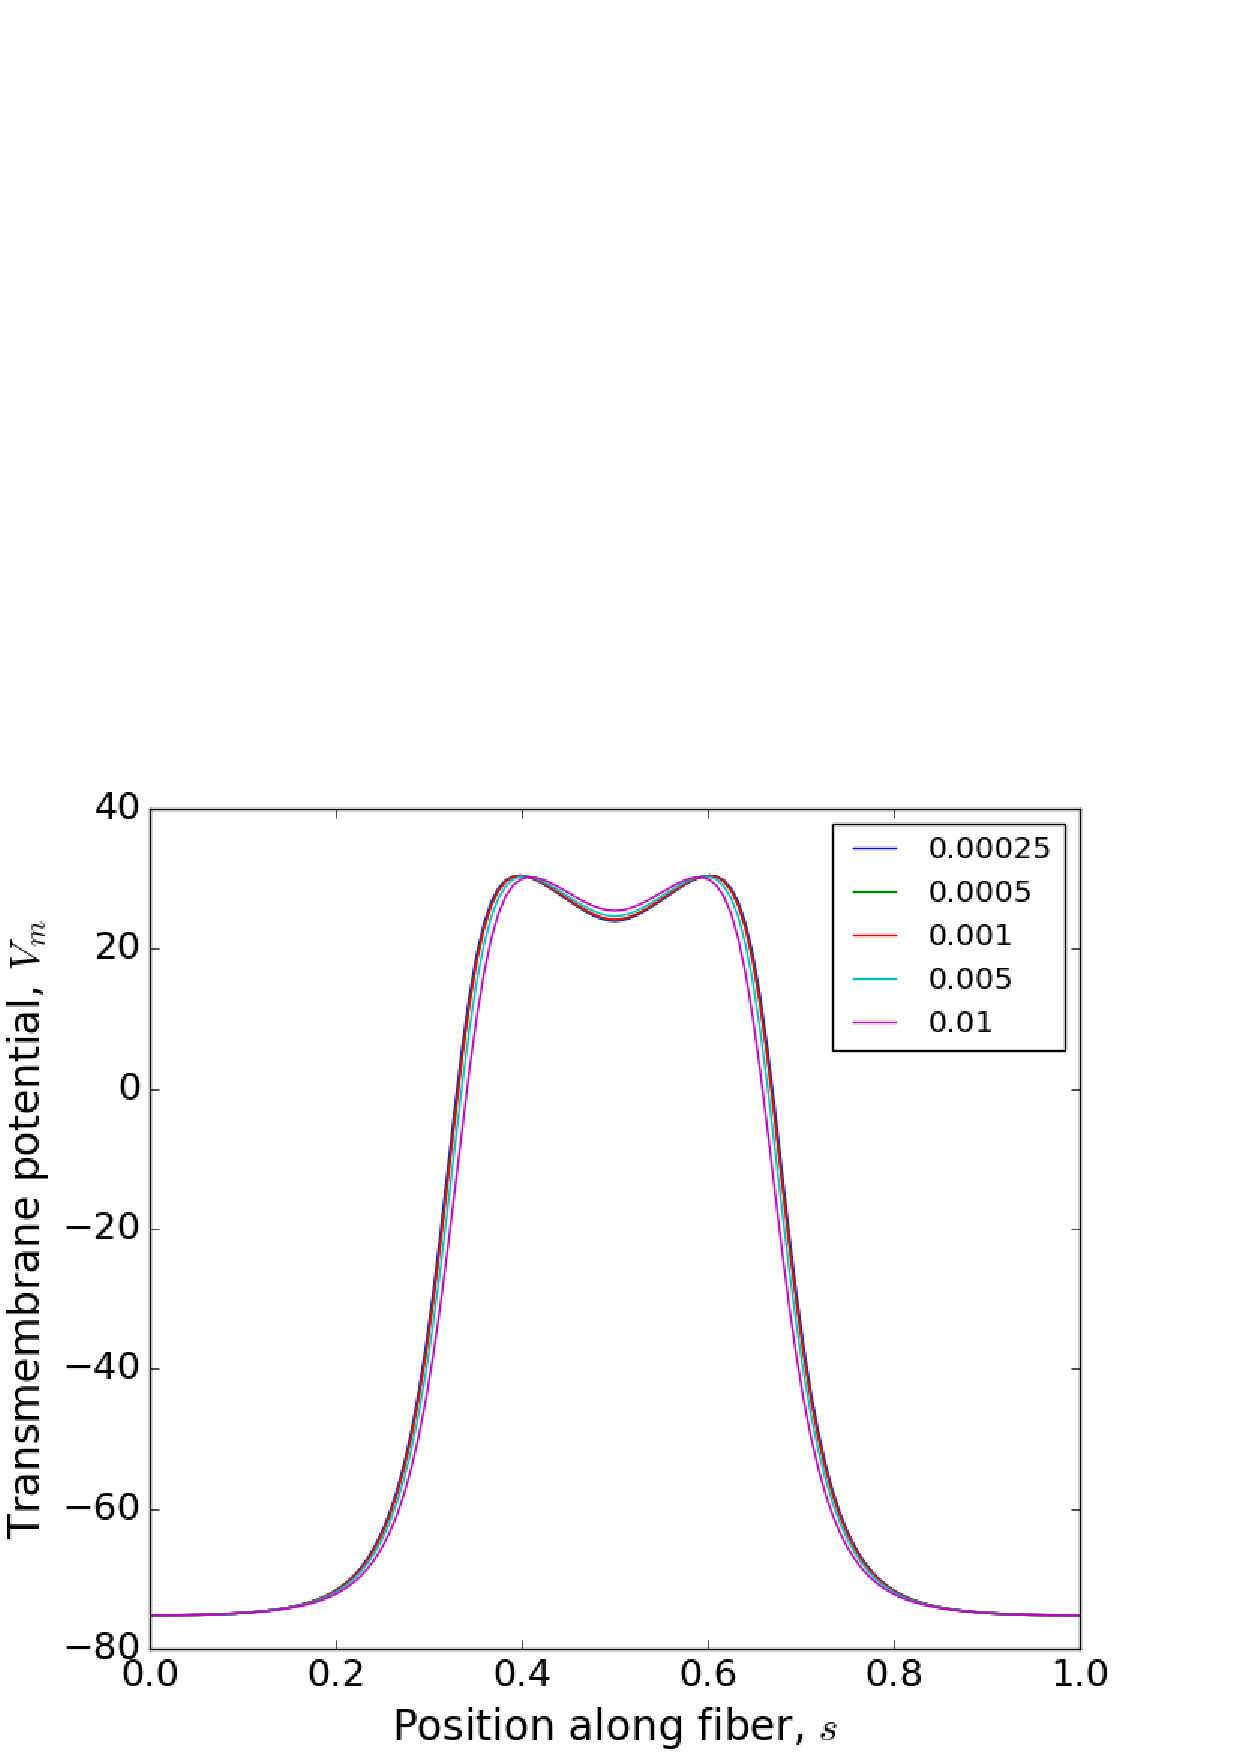
\includegraphics[width=0.9\columnwidth]{examples/example-0404-c/doc/figures/image-Time-Conv-n64-t3.0.png} 
    \caption{$V_m$ for time $t=3.0$, different time step widths d${dt \in \{0.01, 0.005, 0.001, 0.0005, 0.00025\}}$}
    \label{example-0404-c-vm-3.0}
\end{figure}
%
\begin{figure}[h!]
    \centering 
    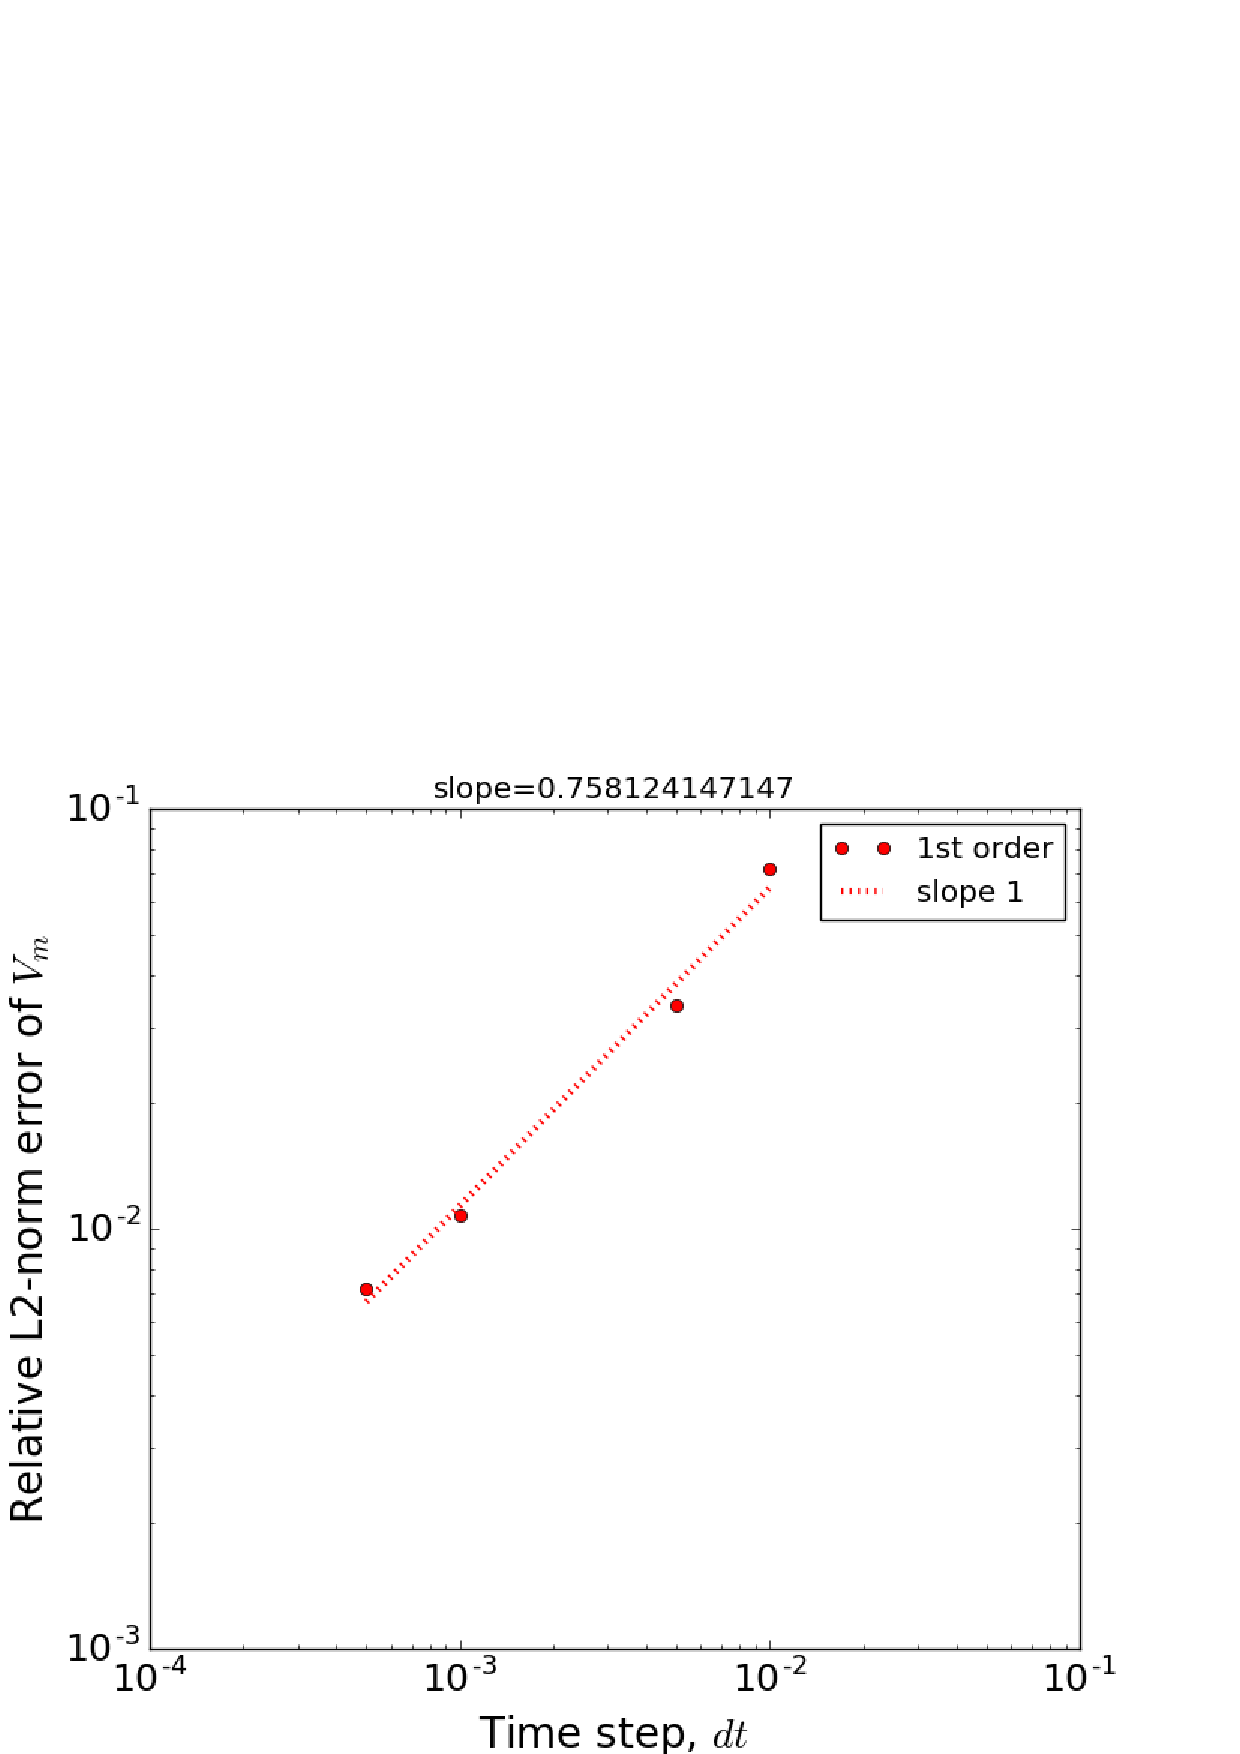
\includegraphics[width=0.9\columnwidth]{examples/example-0404-c/doc/figures/errL2-Time-Conv-n64-t3.0.png} 
    \caption{Error at $t=3.0$ for different time steps widths}
    \label{example-0404-c-error-3.0}
\end{figure}
%
%
%===============================================================================
%
\subsubsection{Validation}
%
%
%===============================================================================
%===============================================================================
